\chapter{The Owens Valley Radio Observatory Long Wavelength Array}

\begin{figure}
    \centering
    \begin{tabular}{cc}
        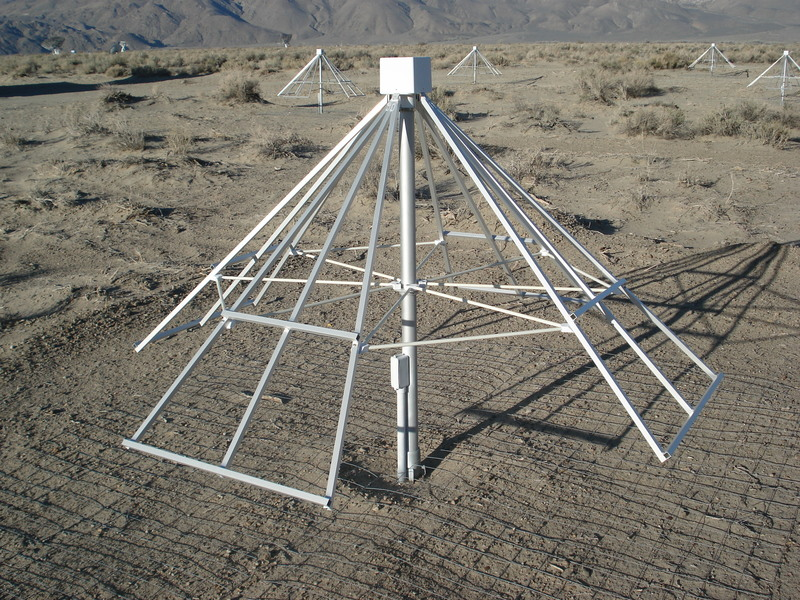
\includegraphics[height=4cm]{figures/chapter2/lwa-antenna} &
        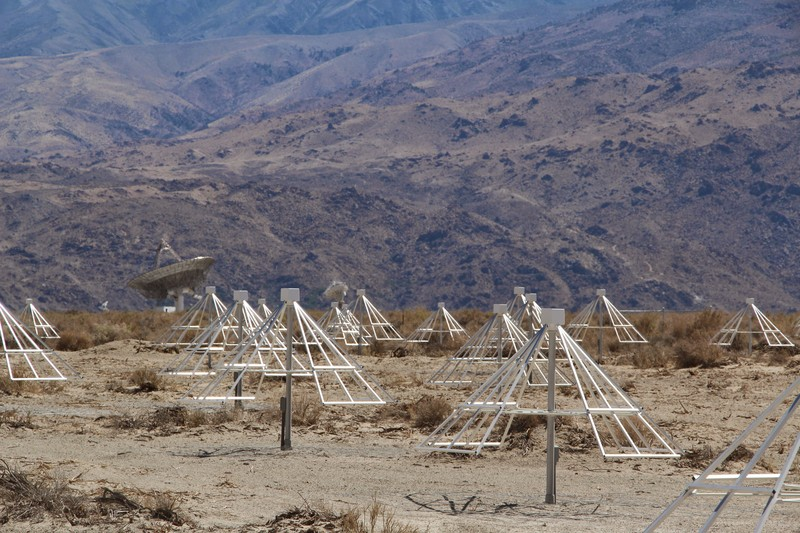
\includegraphics[height=4cm]{figures/chapter2/ovro-lwa} \\
        \textbf{(a)} & \textbf{(b)} \\
    \end{tabular}
    \caption{
        \textbf{(a)} A picture of an OVRO-LWA antenna.
        \textbf{(b)} A view of the OVRO-LWA with the Sierra Mountains in the background.
    }
    \label{fig:ovro-lwa-pictures}
\end{figure}


